% This file was converted to LaTeX by Writer2LaTeX ver. 1.0.2
% see http://writer2latex.sourceforge.net for more info
\documentclass[a4paper,12pt,twoside]{article}
\usepackage[utf8]{inputenc}
\usepackage[T1]{fontenc}
\usepackage[english,ngerman]{babel}
\usepackage{amsmath}
\usepackage{amssymb,amsfonts,textcomp}
\usepackage{array}
\usepackage{hhline}
\usepackage[pdftex]{graphicx}
\pagestyle{headings}
\usepackage{caption2}
\renewcommand{\captionfont}{\small \it}
\renewcommand\figurename{Abb.}

%Obsolete
\newcounter{Abb}
\renewcommand\theAbb{\arabic{Abb}}

\title{efaLive}
\author{Kay Hannay}
\date{2013-07-08}
\begin{document}
\pagenumbering{roman}
%\clearpage\setcounter{page}{1}

\begin{titlepage}
    \vspace*{1cm}
    \begin{center}
        \begin{figure}
            \centering
            
\includegraphics[width=9.745cm,height=7.308cm]{efaLivede-img/efaLivede-img1.png}
        \end{figure}
        \Huge
        {\bf efaLive} \\[0.1cm]
        \LARGE
        Anleitung \\[5cm]
    \end{center}
    \normalsize
    {\bf Datum:} 08.07.2013 \\
    {\bf Version:} 1.4 \\
    {\bf efaLive:} 2.1-2.1.0\_00-x86 \\
    {\bf Kay Hannay} <klinux@hannay.de> \\
\end{titlepage}

%\clearpage\setcounter{page}{1}
%\bigskip

%\setcounter{tocdepth}{10}
%\renewcommand\contentsname{Inhaltsverzeichnis}
\tableofcontents
%\section{}
\pagenumbering{arabic}
\clearpage\setcounter{page}{1}
\section{Einführung}
Diese Anleitung beschreibt, wie man die efaLive-CD benutzt und was man
mit ihr machen kann. Eine Live-CD ist eine CD, von der Computer
gestartet werden können. Das System läuft komplett von der CD und lässt
die Festplatte unangetastet. Daher eignen sich solche Live-CDs
besonders für Demos von Software, Installationen oder auch für
Reparaturen an der Software auf der Festplatte des Computers.

Ein weiteres Merkmal von Live-CDs ist, dass alle Änderungen, die während
des Betriebs vorgenommen wurden, nach dem Herunterfahren des Systems
verloren gehen. Da die Festplatte nicht angetastet wird und eine CD-ROM
nicht beschreibbar ist, gibt es keine Möglichkeit, veränderte Daten
über einen Neustart des Computers hinweg zu speichern. Mit Hilfe eines
USB-Speicher-Sticks kann man dieses Problem jedoch umgehen. Näheres
dazu später.

Das Betriebssystem, welches der CD zugrunde liegt und im Falle einer
Installation auch installiert wird, ist Debian GNU/Linux \cite{DEB1}.
Da es sich bei Linux um Open-Source-Software handelt, fallen keine
Linzenzkosten an. Aufgrund dieser Tatsache ist es überhaupt möglich,
diese Live-CD anzubieten. Mit Microsoft Windows wäre das aus
rechtlichen Gründen nicht möglich.

Das gleiche gilt für die Software efa \cite{EFA1}, die ebenfalls
Open-Source ist und um die es bei dieser Live-CD geht.

\bigskip
ACHTUNG: Auch wenn die hier beschriebene efaLive-CD die Festplatte des
Computers nicht verändert, so kann doch nicht gänzlich ausgeschlossen
werden, dass das Verhalten des Computers durch die Benutzung der
Live-CD in irgendeiner Weise beeinflusst wird. Ich möchte ausdrücklich
darauf hinweisen, dass die Benutzung der CD auf eigene Gefahr erfolgt
und ich für Schäden, die an Hard- und/oder Software entstehen, nicht
hafte.


\bigskip

\section[efaLive{}-CD]{efaLive{}-CD}
\subsection[Hardwarevoraussetzungen]{Hardwarevoraussetzungen}
Dies sind die Hardwareanforderungen, wenn man die Live-CD benutzen
möchte. Die Angaben sind als Minimalvoraussetzung zu verstehen.


\bigskip

{}- Intel Pentium III Prozessor mit 600MHz

{}- 128 MB Arbeitsspeicher

{}- CD-ROM Laufwerk oder USB Anschluss

{}- Monitor mit einer Auflösung von 1024x768 Pixeln

{}- ggf. USB Anschluss für die Datensicherung


\bigskip

\subsection[efaLive{}-CD erstellen]{efaLive{}-CD erstellen}
efaLive kann im Internet unter \cite{EFA4} als ISO CD Abbild
heruntergeladen werden. Um aus dem CD Abbild eine CD zu erstellen,
bieten fast alle Brennprogramme einen Menüpunkt {\textquotedbl}Abbild
brennen{\textquotedbl}, {\textquotedbl}Write CD image{\textquotedbl}
oder ähnlich. Für weitere Informationen bitte die Dokumentation des
\ entsprechenden Programms konsultieren. 

Alternativ kann efaLive auch auf einen USB Stick kopiert werden.

\subsection[Oder per USB Stick]{Oder per USB Stick}
Seit Version 1.2 kann efaLive auch auf einen USB Stick kopiert werden.
Der Computer muss allerdings in der Lage sein, von einem USB Stick zu
starten, was gerade bei älteren Computern nicht unbedingt der Fall ist.


\bigskip

Unter Linux kann das ISO Abbild mit dem Befehlt {\textquotedbl}dd
if={\textless}EFA LIVE ISO{\textgreater} of=/dev/sdb{\textquotedbl}
(wenn /dev/sdb der USB Stick ist) kopiert werden. Achtung: wenn für of=
das falsche Gerät ausgewählt wird, werden womöglich ungewollt Daten
gelöscht!


\bigskip

Unter Windows kann das Programm Win32 Disk Imager \cite{IMG1} verwendet
werden. Da dieses Programm nur Dateien mit der Endung
{\textquotedbl}.img{\textquotedbl} verarbeitet, muss das ISO Abbild
entweder umbenannt werden oder in dem Feld
{\textquotedbl}Dateiname{\textquotedbl} des Programms
{\textquotedbl}*.iso{\textquotedbl} eingegeben werden.


\bigskip

Ansonsten gelten die gleichen Bedingungen, wie bei einer CD.


\bigskip

\subsection[efaLive ausführen]{efaLive ausführen}
Der Start von efaLive ist ganz einfach:


\bigskip

1) CD in das CD-ROM Laufwerk des Computers einlegen oder USB Stick
einstecken

2) Computer (neu) starten

3) In dem Auswahl-Bildschirm (Abb.~\ref{seq:refAbb0}) den Punkt
{\textquotedbl}efaLive{\textquotedbl} (Deutsch oder Englisch) auswählen

\ \ \ \ ({\textless}Enter{\textgreater} drücken)


\bigskip

Bei dem Start wird automatisch efa mit der Bootshausoberfläche geöffnet.
Weitere Informationen zur Benutzung von efa sind in der Dokumentation
zu efa zu finden \cite{EFA2}.


\bigskip


\bigskip


\begin{figure}[htbp]
\centering
\fbox{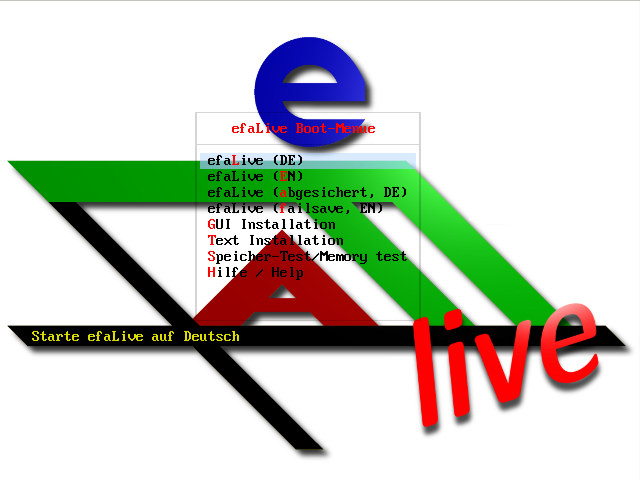
\includegraphics[width=12.012cm,height=9.008cm]{efaLivede-img/efaLivede-img2.png}}
\caption{Auswahlbildschirm Bootloader (Syslinux)}
\label{fig_syslinux}
\end{figure}

%\begin{figure}
%\centering
%\begin{minipage}{12.012cm}
%Abb. {\refstepcounter{Abb}\theAbb\label{seq:refAbb0}}: Auswahlbildschirm
%Bootloader (Syslinux)
%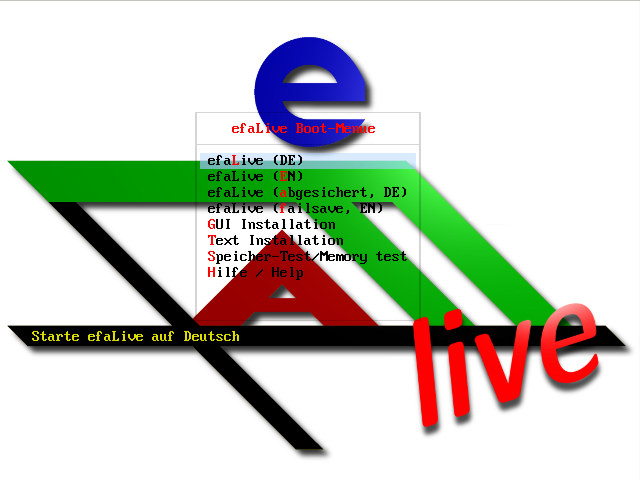
\includegraphics[width=12.012cm,height=9.008cm]{efaLivede-img/efaLivede-img2.png}\end{minipage}
%\end{figure}
Nach einer Weile sollte ein Fenster wie in Abb.~\ref{seq:refAbb1} zu
sehen auf dem Bildschirm erscheinen. Hier kann die Version von efa, die
benutzt werden soll, ausgewählt werden. Ich empfehle an dieser Stelle
efa 2 auszuwählen, da efa 1 nicht mehr gewartet wird und efa 2 viele
Vorteile bietet. Nach der Auswahl auf "`Ok"' klicken.

Das Fenster efaLive Setup kann, wenn efa läuft, jederzeit durch drücken
der Tastenkombination
{\textless}Strg{\textgreater}+{\textless}F12{\textgreater} aufgerufen
werden, um die Einstellung wieder zu ändern. Vor dem Öffnen von efaLive
Setup muss das Passwort des Benutzers {\textquotedbl}efa{\textquotedbl}
eingegeben werden (Die Zeicheneingabe wird nicht durch Ausgaben auf dem
Bildschirm bestätigt). Damit eine Änderung der Version von efa wirksam
wird, muss der Computer in diesem Fall neu gestartet werden.


\bigskip

Das Standard-Passwort vom Benutzer {\textquotedbl}root{\textquotedbl}
ist {\textquotedbl}livecd{\textquotedbl}, das von
{\textquotedbl}efa{\textquotedbl} ist
{\textquotedbl}efalive{\textquotedbl}.


\bigskip


\bigskip


\bigskip



\begin{figure}
\centering
\begin{minipage}{9.006cm}
Abb. {\refstepcounter{Abb}\theAbb\label{seq:refAbb1}}: efaLive Setup
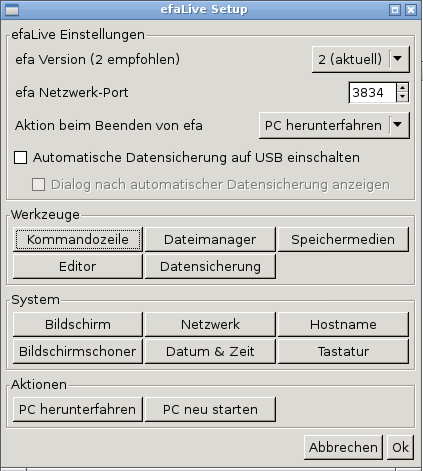
\includegraphics[width=9.006cm,height=10.028cm]{efaLivede-img/efaLivede-img3.png}\end{minipage}
\end{figure}
\subsection{Daten sichern im Live-Betrieb}
Um Änderungen abzuspeichern, kann man einen USB Stick nutzen. Dazu
einfach einen beliebigen USB Stick nehmen und die Datei persistence.zip
aus dem Verzeichnis snapshot der CD auf diesen entpacken, so dass im
Hauptverzeichnis des Sticks die Datei persistence liegt. Den Stick nun
vor dem Start des Computers in einen freien USB Steckplatz stecken und
danach mit der efaLive-CD starten. Während des Startvorgangs sollte der
Stick vom System erkannt und automatisch zum Abspeichern von
sogenannten Snapshots genutzt werden. Dies bedeutet, dass der Inhalt
der Datei persistence beim Start des Computers in das Heimatverzeichnis
des Benutzers {\textquotedbl}efa{\textquotedbl} kopiert wird. In dem
Heimatverzeichnis befinden sich die Konfigurations- und Benutzerdaten
von efa. 

Sobald der Computer heruntergefahren wird, wird der Inhalt des
Heimatverzeichnisses wieder in die Datei persistence kopiert. Es findet
also nur beim Start und beim Herunterfahren des Computers eine
Kopieraktion statt. Daher sollte man den USB Stick erst wieder
entfernen, wenn der Computer vollständig heruntergefahren wurde.


\bigskip

\section{Installation}
\subsection{Hardwarevoraussetzungen}
Auch hier gilt, dass sich die Angaben als Minimalanforderungen
verstehen.


\bigskip

{}- Intel Pentium III Prozessor mit 600MHz

{}- 128 MB Arbeitsspeicher

{}- 2 GB Festplatte

{}- CD-ROM Laufwerk oder USB Anschluss (nur für Installation)

{}- Monitor mit einer Auflösung von 1024x768 Pixeln

{}- ggf. USB Anschluss für die Datensicherung


\bigskip

Der Arbeitsspeicher kann evtl. noch geringer gewählt werden. In diesem
Fall ist jedoch keine grafische Installation mehr möglich. Die
Installation im Text-Modus ist zwar auch nicht sehr schwierig, wird
jedoch in diesem Dokument nicht betrachtet.

Vor der Installation macht es Sinn, sich bereits darüber Gedanken zu
machen, welche Hardwarekomponenten zum Betrieb des Systems wirklich
benötigt werden. Eine Anregung gibt Kapitel 7.1.


\bigskip

\subsection{Die Installationsschritte}
In dieser Beschreibung kann ich leider nur auf bestimmte Aspekte der
Installation eingehen. Ich gehe davon aus, dass ein einfacher
Desktop-PC mit einer Festplatte, einem CD-Rom Laufwerk und optional
einer Netzwerkkarte für kabelgebundene Netzwerke zum Einsatz kommt.
Ferner nehme ich an, dass die komplette Festplatte des Systems gelöscht
werden kann. Weitere (allgemeinere) Informationen zur Installation von
Debian GNU/Linux gibt es unter \cite{DEB2}.


\bigskip

ACHTUNG: Bei der Installation nach dieser Anleitung wird die gesamte
Festplatte des Computers gelöscht! Es gehen also alle auf der
Festplatte gespeicherten Daten verloren! Es ist möglich, dieses
Verhalten zu beeinflussen, jedoch wird darauf in dieser Anleitung nicht
näher eingegangen.


\bigskip


\bigskip



\begin{figure}
\centering
\begin{minipage}{11.494cm}
Abb. \stepcounter{Abb}{\theAbb}: Auswahl der Sprache
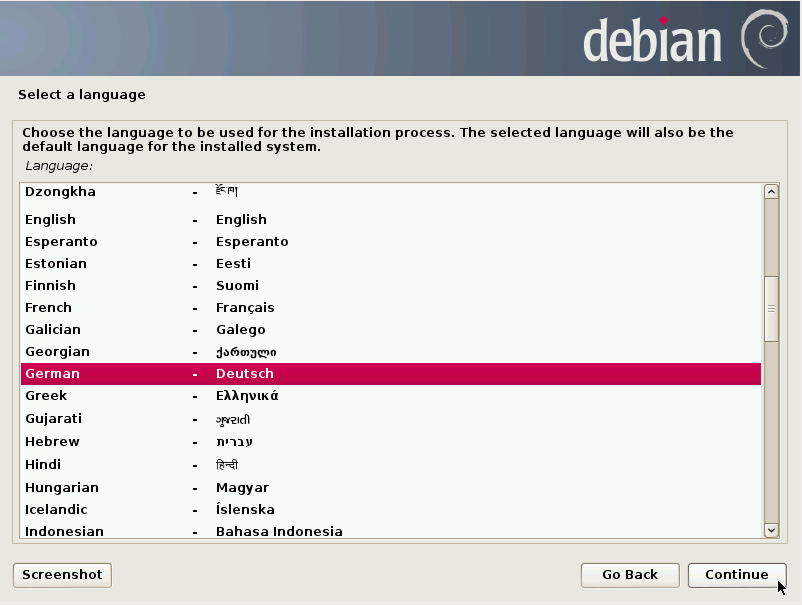
\includegraphics[width=11.494cm,height=8.67cm]{efaLivede-img/efaLivede-img4.png}\end{minipage}
\end{figure}
Im ersten Schritt muss die Sprache gewählt werden. Danach auf den Knopf
{\textquotedbl}Continue{\textquotedbl} klicken. Die Auswahl des
Standortes und der Tastatur kann in den meisten Fällen ohne weitere
Aktion mit einem Klick auf den Knopf
{\textquotedbl}Weiter{\textquotedbl} bestätigt werden.

Bei den nächsten zwei Schritten wird nach dem Land und dem verwendeten
Tastaturlayout gefragt, diese entsprechend beantworten und auf
{\textquotedbl}Weiter{\textquotedbl} klicken..


\bigskip

Computer ohne Netzwerkkarte


\bigskip



\begin{figure}
\centering
\begin{minipage}{11.25cm}
Abb. \stepcounter{Abb}{\theAbb}: Auswahl Netzwerkkarte
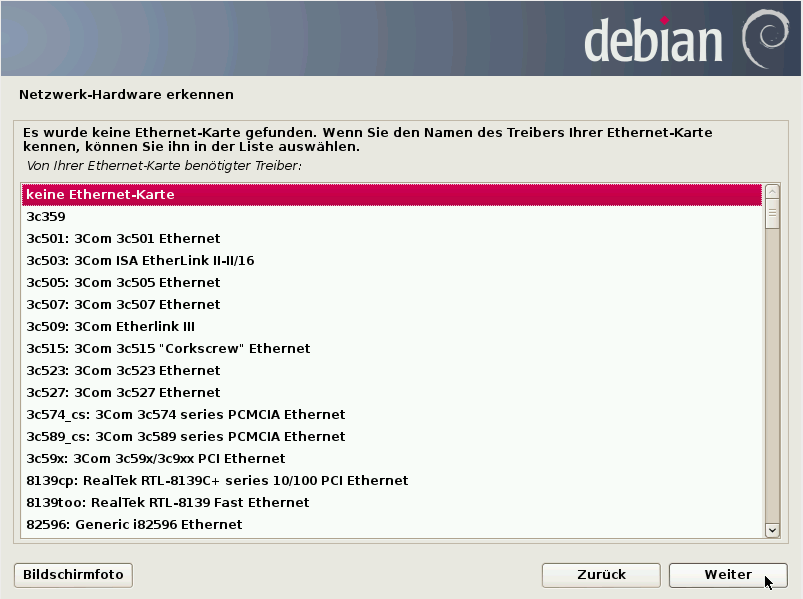
\includegraphics[width=11.25cm,height=8.391cm]{efaLivede-img/efaLivede-img5.png}\end{minipage}
\end{figure}
Da heutige Computer meistens eine Netzwerkkarte besitzen, versucht das
Installationsprogramm recht energisch, eine solche zu finden. Wähle den
Punkt {\textquotedbl}keine Netzwerkkarte{\textquotedbl} aus.


\bigskip


\bigskip



\begin{figure}
\centering
\begin{minipage}{11.25cm}
Abb. \stepcounter{Abb}{\theAbb}: Bestätigung Netzwerkkarte
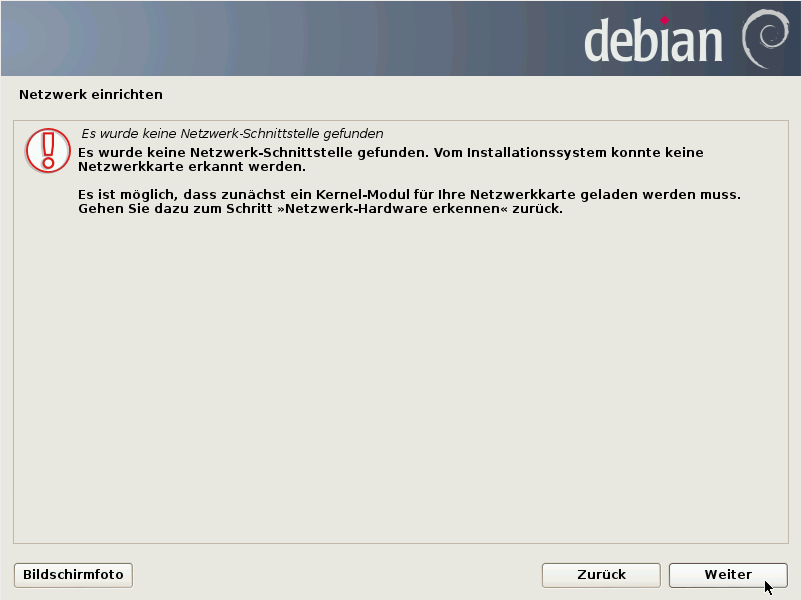
\includegraphics[width=11.25cm,height=8.426cm]{efaLivede-img/efaLivede-img6.png}\end{minipage}
\end{figure}
Es folgt ein Warnhinweis, dass keine Netzwerkkarte gefunden wurde. Diese
kann bestätigt werden. Der nächste Abschnitt kann nun übersprungen
werden.


\bigskip

Computer mit Netzwerkkarte

In der Regel gibt es in den üblichen Netzwerken mit DSL Anschluss oder
ähnlichem auch einen DHCP Server. Dieser Konfiguriert die Netzwerkkarte
automatisch mit den nötigen Einstellungen für das Netzwerk. Meist läuft
ein solcher DHCP Server auf dem Router. Falls die automatische
Konfiguration nicht gelingt, erscheint ein Hinweis, wie in
Abb.~\ref{seq:refAbb5} zu sehen. Andernfalls wird die Konfiguration
automatisch erledigt und es kann mit der Einrichtung der Festplatte
fortgefahren werden.


\bigskip


\bigskip



\begin{figure}
\centering
\begin{minipage}{11.197cm}
Abb. {\refstepcounter{Abb}\theAbb\label{seq:refAbb5}}: Netzwerk konnte
nicht per DHCP konfiguriert werden
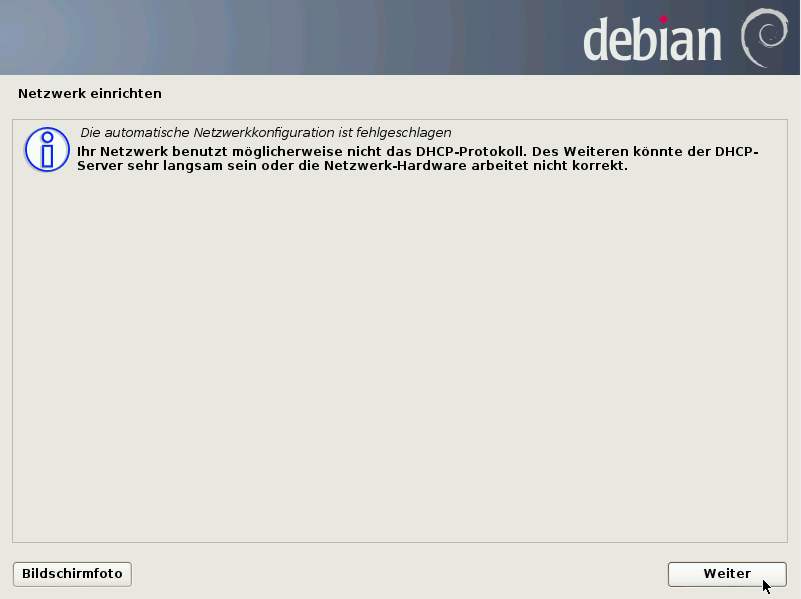
\includegraphics[width=11.197cm,height=8.373cm]{efaLivede-img/efaLivede-img7.png}\end{minipage}
\end{figure}
Dieser Hinweis kann bestätigt werden. Im folgenden Fenster muss nun
ausgewählt werden, wie das Netzwerk zu konfigurieren ist. Ist die
automatische Konfiguration per DHCP fehlgeschlagen, obwohl in dem
Netzwerk ein DHCP Server existiert, muss man sich nun auf die
Fehlersuche begeben und die automatische Konfiguration wiederholen.

Eine andere Möglichkeit ist, das Netzwerk unkonfiguriert zu lassen, was
ich jedoch nicht für sehr sinnvoll erachte, da man in diesem Fall die
Netzwerkkarte besser gleich ausbauen oder deaktivieren sollte (siehe
Kapitel \ref{bkm:RefHeading173029115634}).


\bigskip


\bigskip



\begin{figure}
\centering
\begin{minipage}{11.13cm}
Abb. {\refstepcounter{Abb}\theAbb\label{seq:refAbb6}}: Manuelle
Konfiguration des Netzwerks
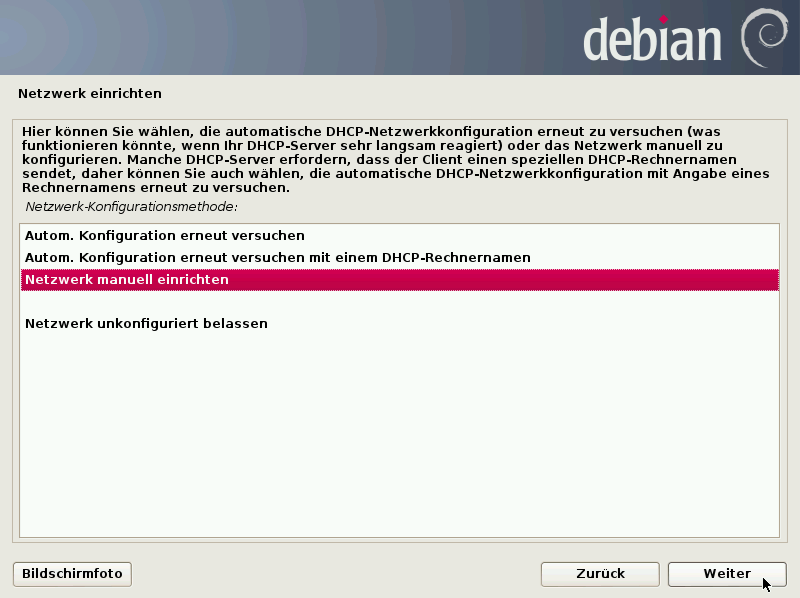
\includegraphics[width=11.13cm,height=8.319cm]{efaLivede-img/efaLivede-img8.png}\end{minipage}
\end{figure}
In der Regel wird man nun das Netzwerk manuell einrichten wollen. Dazu
den entsprechenden Eintrag wie in Abb.~\ref{seq:refAbb6} auswählen und
mit {\textless}Enter{\textgreater} bestätigen. In den nun folgenden
Fenstern werden nacheinander die IP Adresse für den Computer, die
Netzmaske, das Gateway und der Nameserver (DNS) für das Netzwerk
abgefragt. Diese Daten bitte unbedingt gewissenhaft eingeben. Eine
falsche Konfiguration kann das gesamte Netzwerk zum Erliegen bringen.


\bigskip

Festplatte einrichten


\bigskip



\begin{figure}
\centering
\begin{minipage}{11.261cm}
Abb. \stepcounter{Abb}{\theAbb}: Auswahl Partitionierung
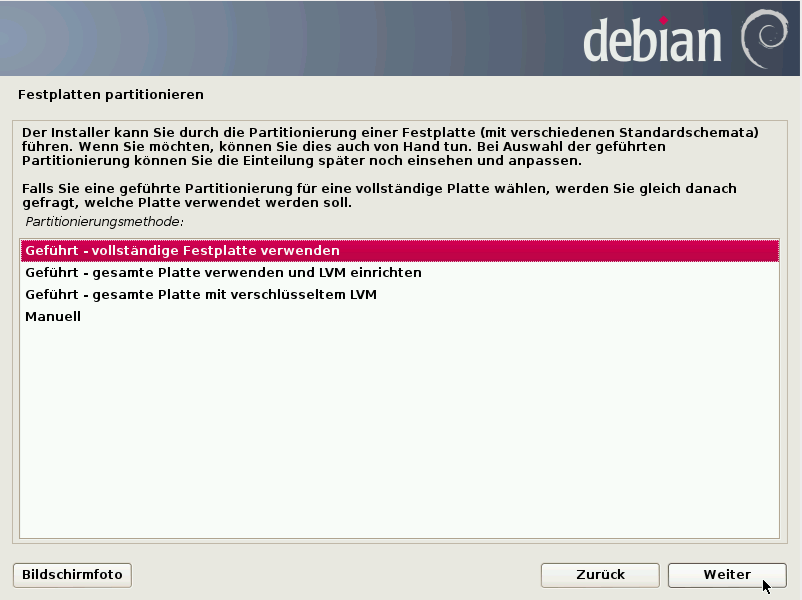
\includegraphics[width=11.261cm,height=8.424cm]{efaLivede-img/efaLivede-img9.png}\end{minipage}
\end{figure}
Im nächsten Schritt wird die Festplatte partitioniert. Das bedeutet,
dass die Festplatte passend für die Benutzung von efa aufgeteilt wird.
Ich gehe hier davon aus, dass die gesamte Festplatte verwendet werden
soll. Dadurch werden alle Daten, die sich auf der Festplatte befinden,
gelöscht! Über den Eintrag {\textquotedbl}Manuell{\textquotedbl} kann
dieses Verhalten beeinflusst werden. Allerdings sollte man sich mit der
Partitionierung von Festplatten auskennen, da sonst ungewollt Daten
verloren gehen können.


\bigskip


\bigskip



\begin{figure}
\centering
\begin{minipage}{11.25cm}
Abb. \stepcounter{Abb}{\theAbb}: Auswahl Festplatte
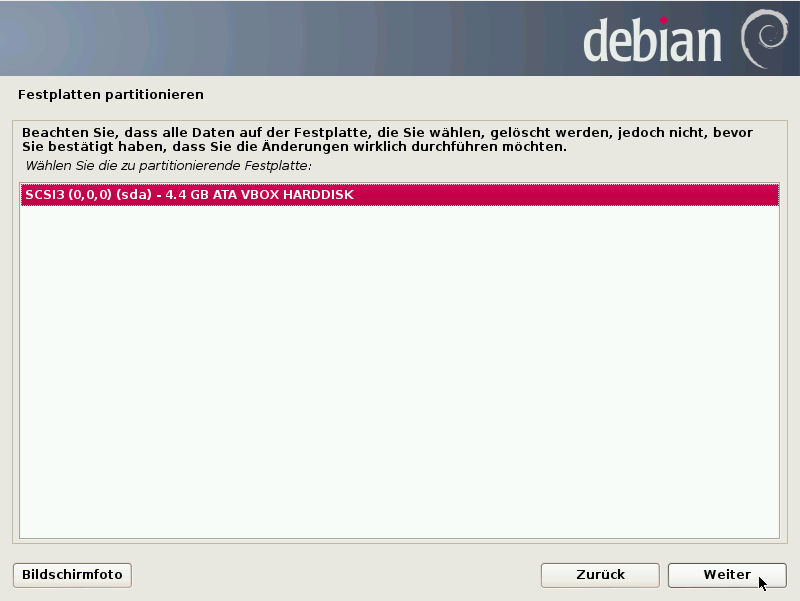
\includegraphics[width=11.25cm,height=8.451cm]{efaLivede-img/efaLivede-img10.png}\end{minipage}
\end{figure}
Als nächstes muss eine Festplatte ausgewählt werden. In diesem Beispiel
befindet sich nur eine Festplatte im Computer, daher kann dieser
Schritt bestätigt werden.


\bigskip


\bigskip



\begin{figure}
\centering
\begin{minipage}{11.261cm}
Abb. \stepcounter{Abb}{\theAbb}: Partitionierung bestätigen
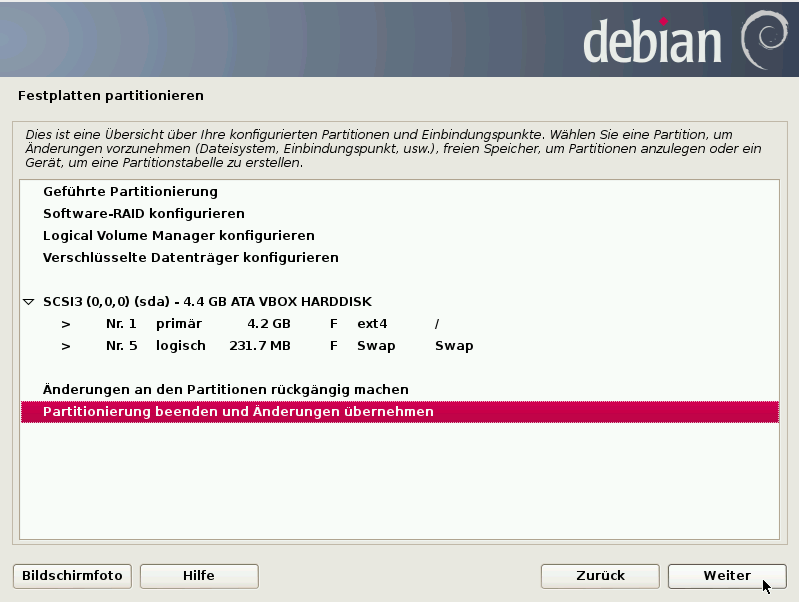
\includegraphics[width=11.261cm,height=8.483cm]{efaLivede-img/efaLivede-img11.png}\end{minipage}
\end{figure}
Es folgt eine Übersicht, wie die Festplatte aufgeteilt werden soll. Mit
{\textquotedbl}Partitionierung beenden und Änderungen
übernehmen{\textquotedbl} geht es weiter.


\bigskip


\bigskip



\begin{figure}
\centering
\begin{minipage}{11.509cm}
Abb. \stepcounter{Abb}{\theAbb}: Sicherheitsabfrage
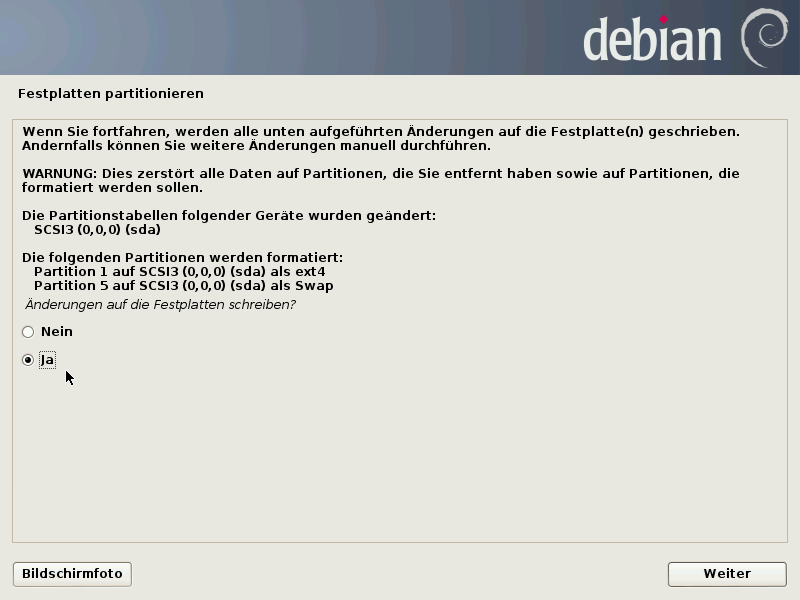
\includegraphics[width=11.509cm,height=8.632cm]{efaLivede-img/efaLivede-img12.png}\end{minipage}
\end{figure}
An dieser Stelle erfolgt noch einmal eine Warnung, dass alle Daten auf
der Festplatte gelöscht werden, wenn dieser Bildschirm mit
{\textquotedbl}Ja{\textquotedbl} bestätigt wird.


\bigskip

Paketverwaltung


\bigskip



\begin{figure}
\centering
\begin{minipage}{11.269cm}
Abb. \stepcounter{Abb}{\theAbb}: Abfrage, ob ein Spiegelserver genutzt
werden soll
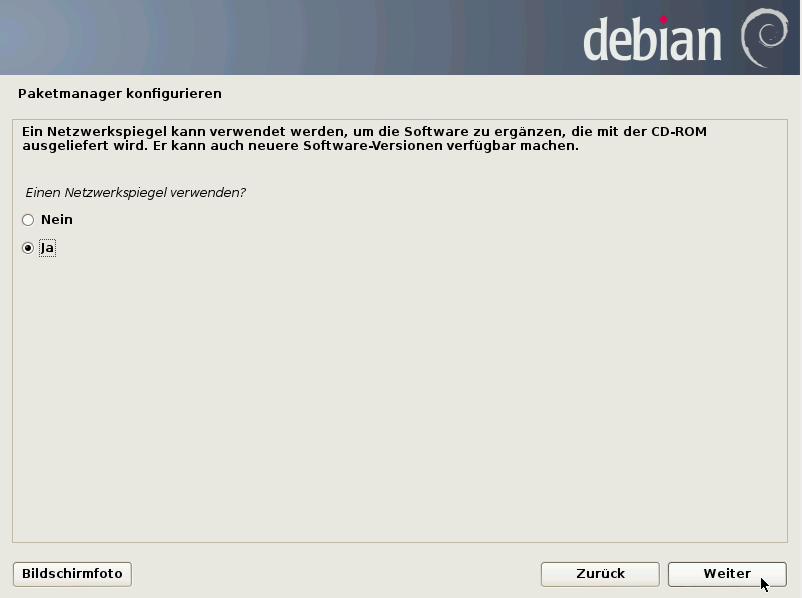
\includegraphics[width=11.269cm,height=8.403cm]{efaLivede-img/efaLivede-img13.png}\end{minipage}
\end{figure}
Das Linux System, welches efaLive zugrunde liegt, kann über das Internet
aktualisiert werden. An dieser Stelle kann nun ein sogenannter
Spiegelserver konfiguriert werden. Verfügt der Computer nicht über eine
Internetverbindung, kann über die Auswahl von
{\textquotedbl}Nein{\textquotedbl} ohne Spiegelserver fortgefahren
werden. Wenn der Computer jedoch über eine Internetverbinsung verfügt,
empfehle ich, einen solchen Server einzurichten.


\bigskip

Spiegelserver sind Server im Internet, die sich in regelmäßigen
Abständen mit dem zentralen Paket-Server des Debian Projekts
abgleichen. Dies dient dazu, den zentralen Server nicht zu überlasten.
Es ist sinnvoll, einen Spiegelserver in der Nähe des eigenen Standortes
auszuwählen, da so tendenziell eine höhere
Datenübertragungsgeschwindigkeit zur Verfügung steht.


\bigskip


\bigskip



\begin{figure}
\centering
\begin{minipage}{11.25cm}
Abb. \stepcounter{Abb}{\theAbb}: Region für Spiegelserver
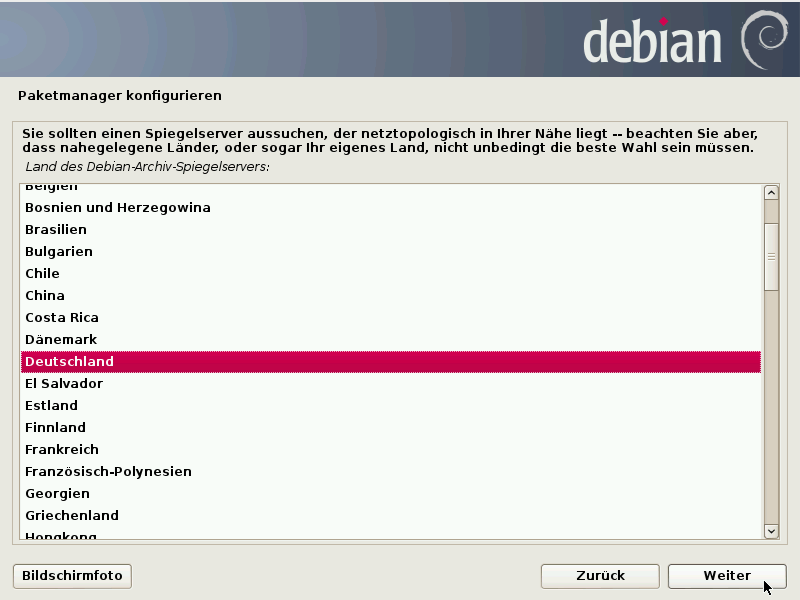
\includegraphics[width=11.25cm,height=8.437cm]{efaLivede-img/efaLivede-img14.png}\end{minipage}
\end{figure}

\bigskip



\begin{figure}
\centering
\begin{minipage}{11.201cm}
Abb. {\refstepcounter{Abb}\theAbb\label{seq:refAbb13}}: Spiegelserver
auswählen
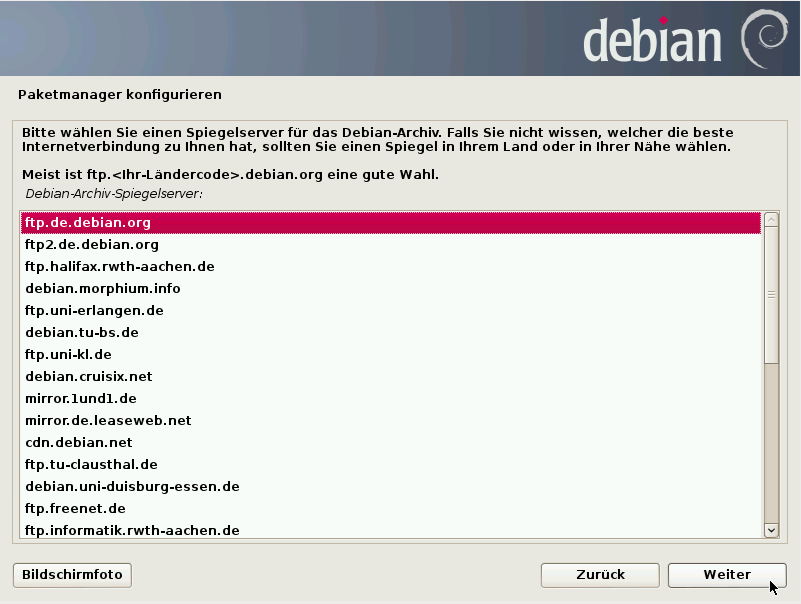
\includegraphics[width=11.201cm,height=8.446cm]{efaLivede-img/efaLivede-img15.png}\end{minipage}
\end{figure}
Ansonsten wird nach einem Klick auf {\textquotedbl}Weiter{\textquotedbl}
ein Dialog wie in Abb.~\ref{seq:refAbb13} angezeigt. Hier kann ein
konkreter Spiegelserver ausgewählt werden. Oft kann man an dem Namen
schon erkennen, ob dieser nah am eigenen Standort steht.


\bigskip


\bigskip



\begin{figure}
\centering
\begin{minipage}{11.25cm}
Abb. \stepcounter{Abb}{\theAbb}: Proxy Server angeben
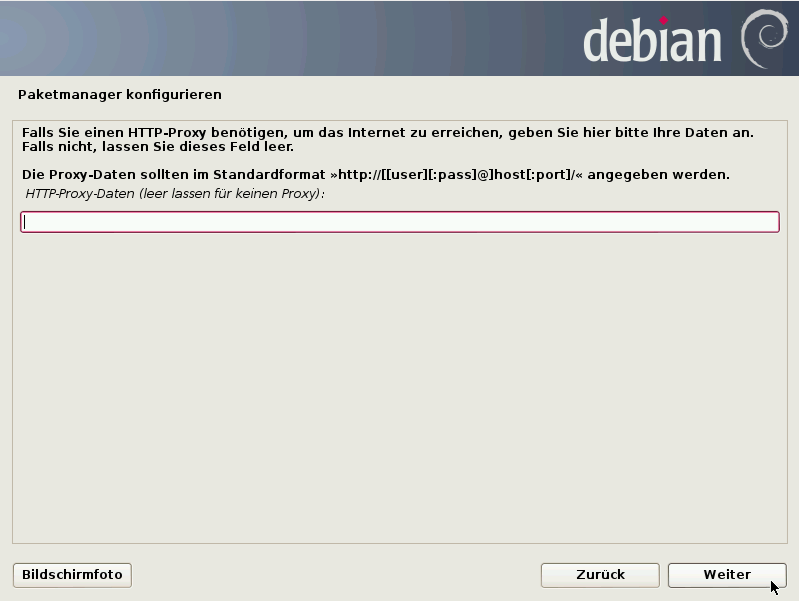
\includegraphics[width=11.25cm,height=8.461cm]{efaLivede-img/efaLivede-img16.png}\end{minipage}
\end{figure}
Es folgt die Abfrage eines Proxy Servers. In den meisten Fällen wird es
keinen geben. Dann kann das Feld leer gelassen werden.


\bigskip


\bigskip

Bootloader


\bigskip



\begin{figure}
\centering
\begin{minipage}{11.269cm}
Abb. \stepcounter{Abb}{\theAbb}: Bootloader Grub installieren
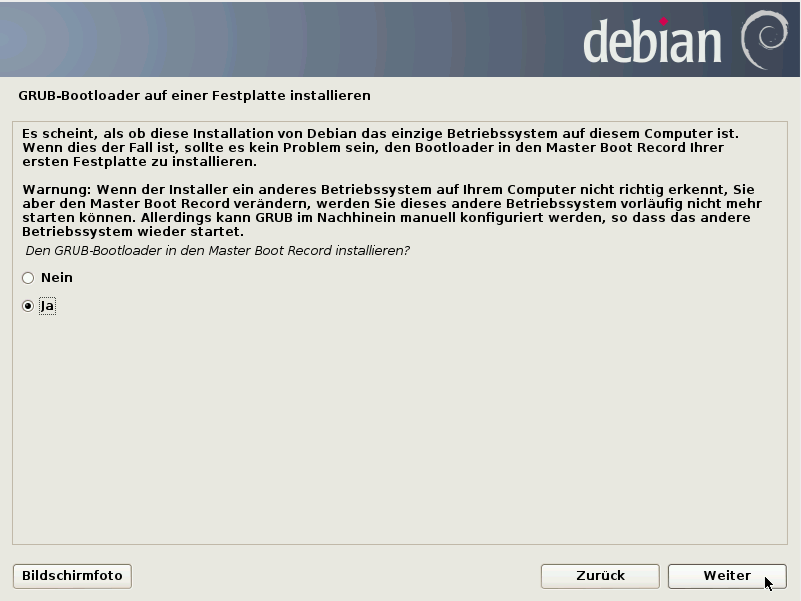
\includegraphics[width=11.269cm,height=8.456cm]{efaLivede-img/efaLivede-img17.png}\end{minipage}
\end{figure}
Nun ist es fast geschafft. Das Installationsprogramm fragt nach, wo der
Bootloader installiert werden soll. Was ein Bootloader ist, spielt an
dieser Stelle keine besondere Rolle. Er sollte jedoch in der Regel im
{\textquotedbl}Master Boot Record{\textquotedbl} installiert werden, da
der Computer das efaLive System sonst nicht automatisch starten wird.
Diesen Dialog also mit {\textquotedbl}Ja{\textquotedbl} bestätigen.


\bigskip


\bigskip



\begin{figure}
\centering
\begin{minipage}{11.261cm}
Abb. \stepcounter{Abb}{\theAbb}: Abschluss
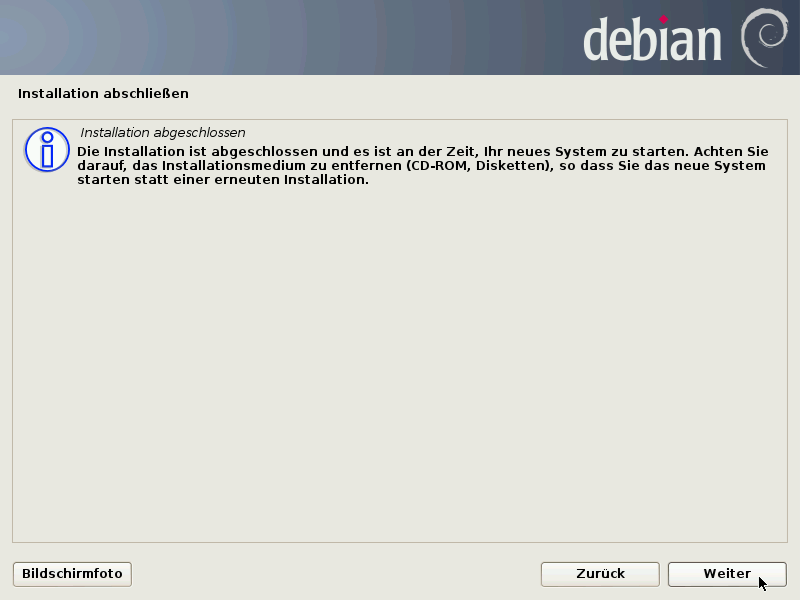
\includegraphics[width=11.261cm,height=8.446cm]{efaLivede-img/efaLivede-img18.png}\end{minipage}
\end{figure}
Es ist geschafft. Die Installation ist vollendet. Wenn Du hier auf
{\textquotedbl}Weiter{\textquotedbl} klickst, wird der Computer neu
gestartet. Damit nicht wieder von der Live-CD gestartet wird, empfiehlt
es sich, diese nun aus dem CD-ROM Laufwerk zu nehmen, bzw. den USB
Stick zu entfernen.


\bigskip

Wenn nun von der Festplatte gestartet wird, erscheint nicht mehr der
Bildschirm wie in Abb.~\ref{seq:refAbb0}. Der gerade installierte
Bootloader tritt nur noch durch eine kurz angezeigte Textzeile in
Erscheinung. An dieser Stelle kann man die {\textless}ESC{\textgreater}
Taste drücken, um in das Menü des Bootloaders zu gelangen. Will man
einen der Einträge in dem Menü editieren, muss man sich
authentifizieren. Die Standardeinstellung ist für den Benutzer
{\textquotedbl}root{\textquotedbl} und für das Passwort
{\textquotedbl}livecd{\textquotedbl}. 

Drückt man keine Taste, startet efaLive. Wie auch beim Start als
Live-CD, kann das Bild, welches während des Starts angezeigt wird, mit
der Taste {\textless}ESC{\textgreater} geschlossen werden, um Meldungen
des Systems angezeigt zu bekommen.


\bigskip

Ich empfehle dringend, Kapitel 7 zu studieren, um das System etwas
sicherer zu machen.


\bigskip

Informationen zur Benutzung von efa gibt es unter \cite{EFA2}.


\bigskip

Viel Spaß mit efaLive!


\bigskip

\section{Administration des Systems}
\subsection[lokaler Zugang]{lokaler Zugang}
\label{bkm:RefHeading31571728}Zur Wartung des Systems wird efaLive-Setup
oder eine Konsole verwendet. Einige Wartungsaufgaben können als
Benutzer {\textquotedbl}efa{\textquotedbl} durchgeführt werden, andere
nur als Benutzer {\textquotedbl}root{\textquotedbl}.

Linux Systeme verfügen über einen Zugang für Administrationsaufgaben.
Der zugehörige Benutzer heißt {\textquotedbl}root{\textquotedbl}.
Meldet man sich als Benutzer {\textquotedbl}root{\textquotedbl} an,
kann man alles an dem System verändern und auch zerstören. Daher sollte
man wirklich nur für Aufgaben, die solche Rechte erfordern, als
Benutzer {\textquotedbl}root{\textquotedbl} arbeiten.


\bigskip

Wenn im folgenden davon gesprochen wird, dass Du dich als
{\textquotedbl}root{\textquotedbl} oder
{\textquotedbl}efa{\textquotedbl} einloggen sollst, dann meint das,
dass Du entweder auf eine der Textkonsolen (Kap.
\ref{bkm:RefHeading14811703288044}) wechseln oder die Konsole der
Toolbox (Kap. \ref{bkm:RefHeading138641045300}) verwenden sollst.


\bigskip

Wenn alle Arbeiten erledigt sind, kann man sich mit dem Befehl
{\textquotedbl}exit{\textquotedbl} (nach Verwendung von
{\textquotedbl}su -{\textquotedbl} 2 Mal) wieder ausloggen. Die Konsole
der Toolbox kann auch per Klick auf das X in der rechten oberen Ecke
des Fensters geschlossen werden.

Diesen Schritt bitte nicht vergessen, denn ansonsten kann ein findiger
Mensch das System ganz leicht manipulieren oder gar löschen.
Gegebenenfalls noch mal mit
{\textless}Alt{\textgreater}+{\textless}Tab{\textgreater} nachsehen, ob
noch ein Fenster im Hintergrund geöffnet ist.


\bigskip

\subsubsection[Toolbox]{Toolbox}
\label{bkm:RefHeading138641045300}Die
{\textquotedbl}Toolbox{\textquotedbl} des efaLive-Setup ist die
bevorzugte Variante eine Konsole aufzurufen. In diesem Fall ist man als
Benutzer {\textquotedbl}efa{\textquotedbl} angemeldet, dessen Passwort
man vor dem Start von efaLive-Setup eingeben muss. Um sich als Benutzer
{\textquotedbl}root{\textquotedbl} anzumelden, muss der Befehl
{\textquotedbl}su -{\textquotedbl} eingegeben werden. Nun erfolgt die
Abfrage des {\textquotedbl}root{\textquotedbl} Passwortes.


\bigskip

Das efaLive-Setup kann jederzeit aus efa heraus über
{\textless}Strg{\textgreater}+{\textless}F12{\textgreater} gestartet
werden. Weitere Informationen zu efaLive-Setup gibt es in Kap.
\ref{bkm:RefHeading14181505831011}.

\subsubsection[Textkonsole]{Textkonsole}
\label{bkm:RefHeading14811703288044}Bei Linux Systemen kann man während
des Betriebs von der grafischen Oberfläche auf Textkonsolen wechseln.
Dies geschieht mit den Tastenkombinationen
{\textless}Strg{\textgreater}+{\textless}Alt{\textgreater}+{\textless}F1{\textgreater}
bis {\textless}F6{\textgreater}. Hinter jeder dieser
Tastenkombinationen verbirgt sich eine Textkonsole, auf der man sich
über einen Benutzernamen und ein Passwort anmelden kann. Um wieder zu
der grafischen Oberfläche zu gelangen, muss man die Tastenkombination
{\textless}Strg{\textgreater}+{\textless}Alt{\textgreater}+{\textless}F7{\textgreater}
drücken. Auf manchen Systemen ist die Verteilung anders geregelt, dann
kann sich die grafische Oberfläche auch hinter
{\textless}Strg{\textgreater}+{\textless}Alt{\textgreater}+{\textless}F1{\textgreater}
verbergen.


\bigskip

Um sich als Benutzer {\textquotedbl}root{\textquotedbl} anzumelden kann
man z.B. mit
{\textless}Strg{\textgreater}+{\textless}Alt{\textgreater}+{\textless}F1{\textgreater}
auf eine Textkonsole wechseln und dort bei
{\textquotedbl}login{\textquotedbl} {\textquotedbl}root{\textquotedbl}
eingeben (und mit {\textless}Enter{\textgreater} bestätigen). Darauf
folgt die Abfrage des Passwortes. Hier ist zu beachten, dass bei der
Eingabe des Passwortes keine Ausgaben auf dem Bildschirm erfolgen. Es
werden also keine Punkte oder Sternchen als Bestätigung der Eingaben
ausgegeben. Bitte nicht verwirren lassen, wenn die Tastatur bis hierher
funktioniert hat, sollte die Eingabe des Passwortes einwandfrei
klappen.


\bigskip

Die Textkonsolen nutzen im Live-Betrieb eine englische Tastatur, daher
ist die Bedienung hier unter Umständen etwas umständlich.

\subsection{Zugang über Netzwerk }
Das efaLive System bringt einen SSH Server mit. SSH ist ein Protokoll,
welches es ermöglicht, sich über das Netzwerk an einem entfernten
Computer anzumelden. Auf Computern mit Linux als Betriebssystem ist die
SSH Client Software normalerweise bereits installiert. Für Windows gibt
es z.B. das Programm Putty \cite{PUT1}.

Unter Linux würde z.B. ein Befehl wie {\textquotedbl}ssh
efa@efalive.efa.local{\textquotedbl} reichen, um eine Konsole auf dem
efaLive Computer zu erhalten, wie sie auch in Kapitel
\ref{bkm:RefHeading31571728} erwähnt ist. In einem kleinen Heimnetzwerk
muss vielleicht nach dem {\textquotedbl}@{\textquotedbl} die IP Adresse
des Rechners verwendet werden, statt des Namens. Aus Sicherheitsgründen
ist es nicht erlaubt, sich direkt als
{\textquotedbl}root{\textquotedbl} Benutzer über SSH anzumelden, daher
habe ich in dem Beispiel den Benutzer {\textquotedbl}efa{\textquotedbl}
verwendet. Um sich als Benutzer {\textquotedbl}root{\textquotedbl}
anzumelden, muss wie bei der Verwendung der Toolbox (Kapitel
\ref{bkm:RefHeading138641045300}) der Befehlt {\textquotedbl}su
-{\textquotedbl} verwendet werden.


\bigskip

Für den Zugriff über das Internet muss in dem verwendeten DSL Router
o.ä. vermutlich eine sogenannte Portweiterleitung eingerichtet werden.
Dabei wird ein beliebiger Netzwerk-Port, z.B. 1234, auf den Port 22 des
efaLive Computers umgeleitet (also dessen Netzwerknamen bzw. IP
Adresse). Aus Sicherheitsgründen sollte der Port auf dem Router (im
Beispiel 1234), der auf den efaLive Computer umgeleitet wird, nicht 22
sein, da dies der Standard-Port für den SSH Dienst ist und hier viele
Angriffsversuche aus dem Internet erfolgen.

Wenn der Zugriff auf das efaLive System vom Internet aus möglich ist,
ist es noch wichtiger, für den Benutzer
{\textquotedbl}efa{\textquotedbl} ein sicheres Passwort zu wählen! Es
sollte möglichst lang sein und Groß-, Kleinbuchstaben, Zahlen und
Sonderzeichen enthalten.


\bigskip

\subsection[Datensicherung]{Datensicherung}
\subsubsection[Sichern]{Sichern}
\label{bkm:RefHeading16481735636932}Das System kann über efaLive-Setup
so eingerichtet werden, dass immer automatisch eine Datensicherung
durchgeführt wird, sobald ein USB Stick in den Computer gesteckt wird. 

Hat die automatische Sicherung funktioniert, ertönen in der Regel drei
kurze Töne. Geht etwas schief, werden 5 lange Töne ausgegeben. In einem
solchen Fall kann man den USB Stick eingesteckt lassen und über den
Dialog {\textquotedbl}Speichermedien{\textquotedbl} der Toolbox eine
Datensicherung durchführen. Fehlermeldungen können hier am Ende über
{\textquotedbl}Details{\textquotedbl} eingesehen werden.

Wurde die erfolgreiche Sicherung durch drei kurze Töne bestätigt, kann
man den Stick herausziehen, er wird nach der Sicherung automatisch
ausgehängt.

Besitzt der PC keinen eingebauten Lautsprecher oder funktionieren die
Tonsignale aus einem anderen Grund nicht, kann in efaLive-Setup ein
Dialog eingeschaltet werden, der nach Beendigung der Datensicherung
angezeigt wird (siehe Kapitel \ref{bkm:RefHeading14181505831011}).


\bigskip

Es sollte sich nun ein Verzeichnis mit dem Namen
{\textquotedbl}efaLive\_backup\_YYYYMMDD\_HHMMSS{\textquotedbl} auf dem
Stick befinden. Wobei YYYYMMDD das aktuelle Datum ist, also z.B.
20100228, und HHMMSS die Uhrzeit, z.B. 134421. In diesem Verzeichnis
befinden sich zwei Dateien,
{\textquotedbl}efa\_backup\_YYYYMMDD\_HHMMSS.zip{\textquotedbl} und
{\textquotedbl}efaLive\_backup\_YYYYMMDD\_HHMMSS.zip{\textquotedbl}.
Erstere Datei enthält die Datensicherung von efa, die Zweite die
Sicherung der efaLive Einstellungen.


\bigskip

Von efaLive werden lediglich einige Einstellungen aus efaLive-Setup
gesichert. Andere Veränderungen am System müssen separat gesichert
werden. Dies ist ein Kompromiss, um möglichst viele Einstellungen zu
speichern, die Datensicherung aber nicht unnötig groß werden zu lassen.



\bigskip

Eine weitere Möglichkeit, eine Datensicherung durchzuführen, ist die
Toolbox, siehe dazu Kapitel \ref{bkm:RefHeading14181505831011}.
Außerdem kann, wie oben beschrieben, der Befehl
{\textquotedbl}efalive-backup{\textquotedbl} benutzt werden.


\bigskip

Hinweis efa 1: Die Datensicherung für efa 1 umfasst lediglich eine Datei
mit dem Namen
{\textquotedbl}efaLive\_backup\_YYYYMMDD\_HHMMSS.zip{\textquotedbl}.


\bigskip

\subsubsection{Wiederherstellen}
Der einfachste Weg, eine Datensicherung zurück zuspielen, ist der
Speichermedien-Dialog (Kapitel \ref{bkm:RefHeading1592839742929}). Hier
kann eine Sicherung direkt von einem USB-Stick wieder eingespielt
werden. Des weiteren kann der Datensicherungs-Dialog (Kapitel
\ref{bkm:RefHeading138841045300}) verwendet werden.


\bigskip

Schließlich kann auch der Schritt der Wiederherstellung an der
Eingabeaufforderung durchgeführt werden. Dazu muss man sich als
Benutzer {\textquotedbl}efa{\textquotedbl} einloggen und den Befehl
{\textquotedbl}efalive-restore
{\textless}DATENSICHERUNG{\textgreater}{\textquotedbl} eingeben. Der
Name der Sicherungsdatei {\textless}DATENSICHERUNG{\textgreater} ist
eine der beiden Sicherungsdateien mit der Endung .zip. Beide Dateien
müssen in einem Verzeichnis liegen. 


\bigskip

Der Computer sollte nach der Wiederherstellung neu gestartet werden,
damit efa die neuen Daten benutzt. Dies kann über efaLive-Setup
erledigt werden.


\bigskip

\section[efaLive{}-Setup]{efaLive-Setup}
\label{bkm:RefHeading14181505831011}efaLive-Setup ist ein Programm, mit
dessen Hilfe verschiedene Einstellungen am efaLive System vorgenommen
werden können. Außerdem enthält efaLive-Setup die
{\textquotedbl}Toolbox{\textquotedbl}, die verschiedene Werkzeuge zur
Verwaltung des efaLive Systems bereitstellt.


\bigskip


\bigskip



\begin{figure}
\centering
\begin{minipage}{9.006cm}
Abb. \stepcounter{Abb}{\theAbb}: efaLive Setup
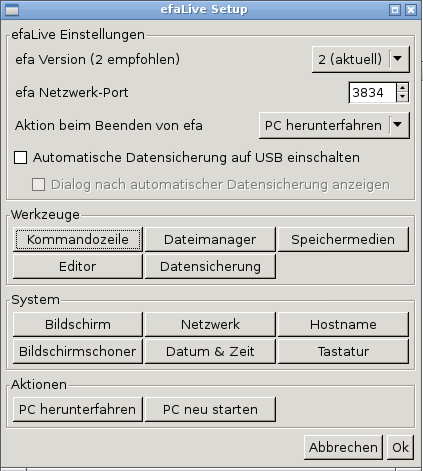
\includegraphics[width=9.006cm,height=10.028cm]{efaLivede-img/efaLivede-img19.png}\end{minipage}
\end{figure}
Mit der Auswahl der efa Version kann man einstellen, ob efa 1 oder efa 2
verwendet werden soll. Diese Einstellung kann auch später noch geändert
werden, nach einem Neustart des Computers startet dann automatisch die
ausgewählte Version.

Der Netzwerk-Port wird nur für efa 2 verwendet. Die Standardeinstellung
3834 muss normalerweise nicht geändert werden. Nur wenn in efa 2 ein
anderer Port eingestellt wurde, muss der Wert hier entsprechend
angepasst werden.


\bigskip

Die {\textquotedbl}Aktion beim Beenden von efa{\textquotedbl} regelt das
Verhalten von efaLive, wenn efa beendet wird. Normalerweise wird der
Computer heruntergefahren. Dies ist jedoch nicht immer gewünscht. Man
kann hier stattdessen einstellen, dass der Computer neu gestartet wird
oder dass nur efa neu gestartet wird.


\bigskip

In der Standardeinstellung ist die automatische Datensicherung auf
USB-Sticks abgeschaltet. Durch das Setzen eines Hakens bei
{\textquotedbl}Automatische Datensicherung auf USB
einschalten{\textquotedbl} kann diese eingeschaltet werden. Ist die
Option aktiv, kann ausgewählt werden, ob nach der automatischen
Datensicherung zusätzlich zu den Tonsignalen ein Dialog angezeigt wird.
Dies ist z.B. nützlich, wenn der Computer keinen Lautsprecher besitzt.

Bitte beachte, dass mit eingeschalteter automatischer Datensicherung im
Prinzip jeder eine Datensicherung machen kann, der einen USB Stick in
den Computer stecken kann. In Konfigurationsdateien etc. sind womöglich
sensible Passwörter gespeichert.


\bigskip

\subsection{Kommandozeile}
Die Kommandozeile, oder auch Textkonsole, kann zu verschiedenen hier im
Dokument beschriebenen Aufgaben verwendet werden. Nach dem Start
arbeitet man als Benutzer {\textquotedbl}efa{\textquotedbl}. Sind
Aufgaben als Benutzer {\textquotedbl}root{\textquotedbl} zu erledigen,
kann man sich über den Befehlt {\textquotedbl}su -{\textquotedbl} als
Benutzer {\textquotedbl}root{\textquotedbl} einloggen.


\bigskip

\subsection{Dateimanager}
Hinter diesem Knopf verbirgt sich ein einfacher Dateimanager. Hier
können Dateien und Verzeichnisse kopiert, verschoben, gelöscht werden,
Dateien mit dem Editor geöffnet werden und vieles mehr.

\subsection[Speichermedien]{Speichermedien}
\label{bkm:RefHeading1592839742929}Will man einen USB-Stick einbinden
oder eine Datensicherung/-wiederherstellung durchführen, kann man
dieses Werkzeug verwenden.


\bigskip



\begin{figure}
\centering
\begin{minipage}{8.375cm}
Abb. \stepcounter{Abb}{\theAbb}: Speichermedien Werkzeug
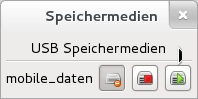
\includegraphics[width=6.212cm,height=3.106cm]{efaLivede-img/efaLivede-img20.png}\end{minipage}
\end{figure}
Es werden untereinander alle gefundenen Speichermedien angezeigt. Dazu
gibt es jeweils drei Knöpfe. Einen zum Ein- und Aushängen des
entsprechenden Mediums. Der Zweite dient dazu, eine Datensicherung auf
dem entsprechenden Speichermedium durchzuführen. Mit dem dritten Knopf
kann eine Datensicherung wiederhergestellt werden. Dazu wird ein Dialog
geöffnet, in dem man eine der beiden Sicherungsdateien auswählen muss.
Wichtig ist hier, dass beide Sicherungsdateien in demselben Verzeichnis
liegen und nicht umbenannt wurden.

Sowohl das Ende der Datensicherung, als auch das Ende der
Wiederherstellung werden durch einen Dialog signalisiert, der auch ggf.
aufgetretene Probleme anzeigt.


\bigskip

Bewegt man den Mauszeiger über den Namen eines Speichermediums und lässt
den Zeiger dort eine Weile verweilen, werden verschiedene Informationen
zu dem Medium angezeigt, unter anderem der Einhängepunkt. Das ist das
Verzeichnis im Dateisystem, wo das Speichermedium nach dem Einhängen zu
finden ist.

Unter Gerät ist der Gerätename zu finden, über den man das
Speichermedium ansprechen kann.


\bigskip

\subsection[Editor]{Editor}
\label{bkm:RefHeading30771485014445}Dieser Knopf startet einen einfachen
grafischen Texteditor namens {\textquotedbl}Leafpad{\textquotedbl}, mit
dem z.B. Konfigurationsdateien editiert werden können. (Siehe auch
Kapitel \ref{bkm:RefHeading2936838803289})


\bigskip

\subsection[Datensicherung]{Datensicherung}
\label{bkm:RefHeading138841045300}Mit diesem Werkzeug können
Datensicherungen erstellt oder wiederhergestellt werden. Der
Mechanismus ist ganz ähnlich zu dem im Speichermedien-Dialog. Nur
können hier Datensicherungen an einer beliebigen Stelle im Dateisystem
erstellt werden.

Nach einem Klick auf den Knopf
{\textquotedbl}Datensicherung{\textquotedbl} öffnet sich ein Dialog, in
dem ein Verzeichnis ausgewählt werden muss. In dieses Verzeichnis wird
die Datensicherung gespeichert. Das Ende der Datensicherung wird durch
einen Dialog angezeigt, der auch mitteilt, ob die Sicherung erfolgreich
war.


\bigskip



\begin{figure}
\centering
\begin{minipage}{5.689cm}
Abb. \stepcounter{Abb}{\theAbb}: Datensicherung
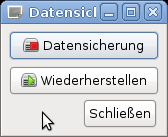
\includegraphics[width=4.445cm,height=3.625cm]{efaLivede-img/efaLivede-img21.png}\end{minipage}
\end{figure}

\bigskip

Klickt man auf {\textquotedbl}Wiederherstellen{\textquotedbl}, öffnet
sich ein Dialog, in dem eine der beiden Sicherungsdateien (.zip)
ausgewählt werden muss. Die beiden Dateien müssen sich in demselben
Verzeichnis befinden und dürfen nicht umbenannt worden sein. Auch hier
wird das Ende der Wiederherstellung durch einen Dialog angezeigt.


\bigskip

\subsection{Bildschirm-Setup}
Dieses Werkzeug kann verwendet werden, um den oder die angeschlossenen
Bildschirme zu konfigurieren.


\bigskip


\bigskip



\begin{figure}
\centering
\begin{minipage}{8.848cm}
Abb. \stepcounter{Abb}{\theAbb}: Bildschirm-Setup Werkzeug
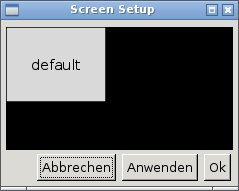
\includegraphics[width=8.431cm,height=6.738cm]{efaLivede-img/efaLivede-img22.jpg}\end{minipage}
\end{figure}
Alle erkannten Bildschirme werden mit Namen versehen als graue Rechtecke
in dem Fenster dargestellt. Klickt man mit der rechten Maustaste auf
einen der Bildschirme, öffnet sich ein Kontextmenü, mit dem man den
betreffenden Bildschirm ein- oder ausschalten, rotieren oder die für
diesen Bildschirm verwendete Auflösung verändern kann. Klickt man mit
der linken Maustaste auf einen Bildschirm und hält die Maustaste
gedrückt, kann man die Bildschirme verschieben. Dadurch kann man
mehrere angeschlossenen Geräte das gleiche Bild anzeigen lassen, oder
auf verschiedene Weisen nebeneinander anordnen.

Ein Klick auf {\textquotedbl}Anwenden{\textquotedbl} übernimmt die
Einstellungen für die aktive Darstellung. Mit einem Klick auf
{\textquotedbl}Ok{\textquotedbl} werden die Einstellungen gespeichert
und bei jedem Start von efaLive automatisch geladen.


\bigskip

\subsection{Netzwerk}
Über diesen Knopf wird ein Programm namens
{\textquotedbl}Network-Manager{\textquotedbl} gestartet. Hier können
alle Netzwerkverbindungen des Rechners verwaltet werden. Auf ein paar
Spezialitäten gehe ich im Folgenden ein. Weitere Dokumentation zu dem
{\textquotedbl}Network-Manager{\textquotedbl} gibt es unter
\cite{NWM1}.



\begin{figure}
\centering
\begin{minipage}{10.82cm}
Abb. \stepcounter{Abb}{\theAbb}: Netzwerk-Einstellungen
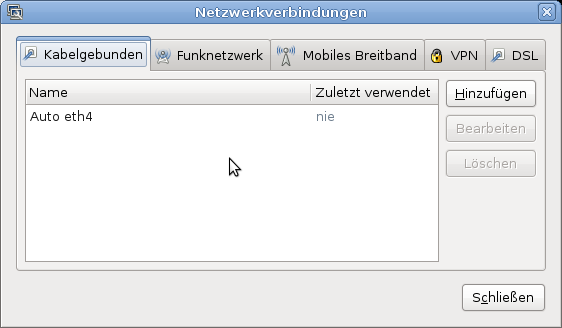
\includegraphics[width=14.87cm,height=8.678cm]{efaLivede-img/efaLivede-img23.png}\end{minipage}
\end{figure}
\subsubsection[W{}-LAN]{W-LAN}
Um eine W-LAN Verbindung hinzuzufügen, auf den Reiter
{\textquotedbl}Funknetzwerk{\textquotedbl} klicken und dort auf den
Knopf {\textquotedbl}Hinzufügen{\textquotedbl} klicken. Einzutragen ist
mindestens die SSID, also der Namen des W-LAN, in den
Sicherheitseinstellungen ist die Verschlüsselung des WLAN auszuwählen,
sowie das zugehörige Passwort einzutragen und {\textquotedbl}Für alle
Benutzer verfügbar{\textquotedbl} auszuwählen. Ggf. kannst Du einen
Haken bei {\textquotedbl}Automatisch verbinden{\textquotedbl} setzen.


\bigskip



\begin{figure}
\centering
\begin{minipage}{11.072cm}
Abb. \stepcounter{Abb}{\theAbb}: W-LAN Einstellungen
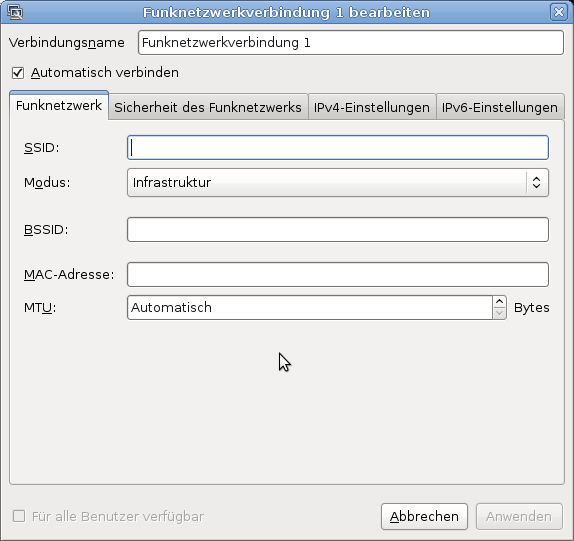
\includegraphics[width=15.187cm,height=14.314cm]{efaLivede-img/efaLivede-img24.png}\end{minipage}
\end{figure}
\subsubsection{Breitband}
Auch Breitbandverbindungen über z.B. UMTS können konfiguriert werden.
Über den Knopf {\textquotedbl}Hinzufügen{\textquotedbl} kann ein
Assistent gestartet werden, der bei der Einrichtung unterstützt.
Zuletzt muss noch ein Haken bei {\textquotedbl}Für alle Benutzer
verfügbar{\textquotedbl} gesetzt und ggf. die PIN eingegeben werden. Da
leider im Fall von Breitbandverbindungen die Option
{\textquotedbl}Automatisch verbinden{\textquotedbl} nicht funktioniert,
bringt efaLive eine Zusatzfunktion dafür mit. Damit diese funktioniert,
muss die Breitandverbindung {\textquotedbl}broadband{\textquotedbl}
heißen. Ist die Verbindung entsprechend eingerichtet, prüft efaLive
alle 5 Minuten, ob der Rechner mit dem Internet verbunden ist und
startet ggf. die Verbindung.


\bigskip

Achtung: Durch die Verwendung einer Breitbandverbindung können unter
Umständen hohe Kosten entstehen. Wenn Du keinen entsprechenden Tarif
hast, solltest Du diese Funktion nicht nutzen.


\bigskip

\subsection[Hostname]{Hostname}
Hinter diesem Knopf verbirgt sich ein Assistent zur Einrichtung eines
dynamischen DNS Dienstes. Ein solcher Dienst sorgt dafür, dass ein
Computer, der über eine Internetverbindung mit wechselnder IP Adresse
verbunden ist, immer mit einen festen Rechnernamen erreichbar ist. Das
ist für den Zugriff auf efa sehr praktisch. Allerdings funktioniert die
Konfiguration in efaLive nur, wenn der Computer direkt mit dem Internet
verbunden ist. Befindet sich noch ein Router dazwischen, muss die
Konfiguration auf diesem durchgeführt werden.


\bigskip

\subsection{Tastatur}
Über diesen Knopf kann die verwendete Tastatur konfiguriert werden. Dies
umfasst sowohl die Einstellungen zum Gerät, als auch die
Tastenbelegung.


\bigskip

\subsection{Bildschirmschoner}
Um die Einstellungen für den Bildschirmschoner, bzw. die
Enegiespareinstellungen für den Bildschirm zu konfigurieren, kann
dieses Programm verwendet werden.


\bigskip

\subsection{Datum und Uhrzeit}
Mit diesem Programm kann die Uhrzeit und das Datum für den Computer
eingestellt werden. Alternativ kann das {\textquotedbl}Network Time
Protocol{\textquotedbl} verwendet werden. Hierbei wird die Zeit über
das Internet synchronisiert. Das funktioniert natürlich nur unter
Verwendung einer Internetverbindung.


\bigskip



\begin{figure}
\centering
\begin{minipage}{6.59cm}
Abb. \stepcounter{Abb}{\theAbb}: Einstellungen Datum \& Uhrzeit
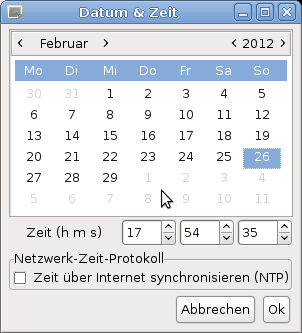
\includegraphics[width=7.99cm,height=8.811cm]{efaLivede-img/efaLivede-img25.png}\end{minipage}
\end{figure}

\bigskip

\subsection[Aktionen]{Aktionen}
Unter Aktionen gibt es aktuell zwei Knöpfe. Einen, um den Computer
herunterzufahren, mit dem anderen kann der Computer neu gestartet
werden. Beide Aktionen müssen noch einmal in einem Dialog bestätigt
werden, damit der Computer nicht unbeabsichtigt heruntergefahren wird.


\bigskip

\section{Software verwalten}
\subsection{efa aktualisieren}
Wenn eine aktuellere Version von efa zum Einsatz kommen soll, ist es
nicht nötig, das komplette System neu zu installieren. Es kann die in
efa eingebaute Funktion zur Aktualisierung verwendet werden. 

Oder man lädt das aktuelle efa von der efa Internetseite \cite{EFA1}
herunter und kopiert es auf einen USB Stick. Diesen USB Stick nun in
einen freien USB Steckplatz des efaLive System einstecken. 

Nun muss man den USB Stick über die Toolbox einbinden und sich wie in
Kapitel 4.1 beschrieben auf einer Textkonsole als Benutzer
{\textquotedbl}efa{\textquotedbl} einloggen und die folgenden Befehle
eingeben:


\bigskip

cd /usr/lib/efa2

unzip -o /media/{\textless}EINHÄNGEPUNKT{\textgreater}/{\textless}NAME
DER EFA DATEI{\textgreater}


\bigskip

{\textless}EINHÄNGEPUNKT{\textgreater} ist hier durch den Namen des USB
Sticks im /media/ Verzeichnis zu ersetzen und {\textless}NAME DER EFA
DATEI{\textgreater} durch den Namen der heruntergeladenen Datei (z.B.
efa2.zip).

Nach einem Neustart des Systems sollte automatisch die neue Version von
efa gestartet werden.


\bigskip

Wird efa 1 benutzt, ist bei den obigen Befehlen nicht \ /usr/lib/efa2,
sondern /usr/lib/efa zu verwenden.


\bigskip

\subsection{Linux Software verwalten}
Um weitere Linux Programme zu installieren oder die installierte
Software (abgesehen von efa) zu aktualisieren, gibt es im Wesentlichen
drei Verfahren. 

Zum einen können Pakete manuell heruntergeladen und installiert werden,
zum anderen kann man Software von Debian CDs installieren. Außerdem
gibt es die Möglichkeit, das efaLive System so zu konfigurieren, dass
es sich auf Anweisung selbst die entsprechende Software herunterlädt.
Dazu muss jedoch von dem System aus das Internet erreichbar sein.

Die Version der hier verwendeten Debian Distribution ist
{\textquotedbl}Wheezy{\textquotedbl}.


\bigskip

\subsubsection{Software manuell installieren}
Es können unter \cite{DEB3} Softwarepakete für das Live-System
heruntergeladen werden. Diese Softwarepakete haben die Endung
{\textquotedbl}.deb{\textquotedbl} und können auf dem efaLive System
über das Programm dpkg installiert werden. Problematisch bei der
manuellen Installation ist, dass es zwischen den einzelnen Paketen
Abhängigkeiten gibt. Wenn also Programm X installiert werden soll, so
benötigt dieses evtl. noch Programm Y. Auf der Internetseite werden
diese Abhängigkeiten zwar angezeigt, man weiß jedoch nicht unbedingt,
welche der Abhängigkeiten bereits installiert sind. Daher ist dieses
Vorgehen nur für kleine Programme zu empfehlen.

An dieser Stelle funktioniert die Vorgehensweise wie in 6.2.4
beschrieben nicht. Hat man eines oder mehrere Pakete heruntergeladen,
werden diese als Benutzer {\textquotedbl}root{\textquotedbl} mit dem
Befehl {\textquotedbl}dpkg -i {\textless}SOFTWARE PAKET 1{\textgreater}
{\textless}SOFTWARE PAKET 2{\textgreater} ...{\textquotedbl}
installiert. 


\bigskip

\subsubsection{Software von CDs}
Unter \cite{DEB4} können CD-Abbilder von der kompletten Debian
Distribution heruntergeladen werden. So steht eine riesige Auswahl an
Software auch ohne Internetzugang zur Verfügung. Je nach Anforderungen
müssen nicht alle CDs heruntergeladen werden. Liegen eine oder mehrere
Debian CDs vor, können diese als Benutzer
{\textquotedbl}root{\textquotedbl} mit dem Befehl
{\textquotedbl}apt-cdrom add{\textquotedbl} dem System bekannt gemacht
werden. Das Programm fordert automatisch zum Einlegen von CDs auf.

Diese Methode ist vorzuziehen, wenn kein Internetzugang für das efaLive
System zur Verfügung steht.


\bigskip

\subsubsection{Software direkt aus dem Internet}
Steht ein Internetzugang zur Verfügung, so ist dies der komfortabelste
Weg, Software zu installieren oder aktualisieren. Stand bereits zum
Zeitpunkt der Installation von efaLive ein Internetzugang, so wurde
wahrscheinlich bereits ein Spiegelserver eingerichtet. Sonst müssen als
Benutzer {\textquotedbl}root{\textquotedbl} die folgenden Befehle
ausgeführt werden:


\bigskip

echo {\textquotedbl}deb http://ftp.de.debian.org/debian/ wheezy main
contrib non-free{\textquotedbl} {\textgreater}{\textgreater}
/etc/apt/sources.list

echo {\textquotedbl}deb-src http://ftp.de.debian.org/debian/ wheezy main
contrib non-free{\textquotedbl} {\textgreater}{\textgreater}
/etc/apt/sources.list


\bigskip

Danach muss der interne Index aktualisiert werden. Dies geschieht über
{\textquotedbl}aptitude update{\textquotedbl}.


\bigskip

\subsubsection[Installieren/Löschen/Suchen/Aktualisieren]{Installieren/Löschen/Suchen/Aktualisieren}
\label{bkm:RefHeading11661832955836}Für die Verwaltung der
Linux-Software kann der Befehl {\textquotedbl}aptitude{\textquotedbl}
benutzt werden. Mit {\textquotedbl}aptitude search
{\textless}STICHWORT{\textgreater}{\textquotedbl} kann nach Paketen
gesucht werden (funktioniert leider nicht immer sehr gut). Um ein Paket
zu installieren genügt ein {\textquotedbl}aptitude install
{\textless}PAKETNAME{\textgreater}{\textquotedbl}, um eines zu löschen
{\textquotedbl}aptitude purge
{\textless}PAKETNAME{\textgreater}{\textquotedbl}. Gegebenenfalls fragt
das Programm aptitude nach, ob z.B. bestimmte Abhängigkeiten
automatisch mit installiert werden sollen.

Soll die installierte Software aktualisiert werden, kann
{\textquotedbl}aptitude safe-upgrade{\textquotedbl} aufgerufen werden.

In jedem Fall sollte vor der Nutzung einer dieser Funktionen ein
{\textquotedbl}aptitude update{\textquotedbl} durchgeführt werden.


\bigskip

\section[Absichern des Systems]{Absichern des Systems}
\label{bkm:RefHeading173029115634}Es empfiehlt sich, den Computer, der
ja \ wahrscheinlich im Bootshaus steht und für viele Menschen
zugänglich ist, ein wenig abzusichern. Daher hier ein paar Tipps, wie
man etwas mehr Sicherheit erreichen kann. Allerdings bieten auch all
diese Hinweise keine absolute Sicherheit. Wer sich gut mit Computern
auskennt, wird auch diese Hürden überwinden können. Es ist trotzdem
nützlich, die Latte möglichst hoch zu legen.


\bigskip

\subsection[Peripherie]{Peripherie}
\label{bkm:RefHeading31562628}Um die Zugangsmöglichkeiten zum System
einzuschränken, sollte man aus dem Computer alle Hardware ausbauen, die
nicht für den Betrieb benötigt wird. Hier eine Liste von Dingen, die
man oft ausbauen kann:


\bigskip

\begin{itemize}
\item Diskettenlaufwerke
\item Netzwerkkarte
\item Soundkarte
\item Karten mit seriellen, parallelen oder sonstigen nicht benötigten
Schnittstellen
\item CD-ROM Laufwerk (nach der Installation wird es normalerweise nicht
mehr benötigt)
\end{itemize}

\bigskip

\subsection{BIOS}
Alles, was nicht physikalisch aus dem Computer ausgebaut werden kann,
aber für den Betrieb von efaLive nicht von Nöten ist, sollte wenigstens
im BIOS des Computers ausgeschaltet werden. Oft gibt es hier die
Möglichkeit, die im Abschnitt 7.1 erwähnten Geräte abzuschalten.
Außerdem kann man meistens das Starten von Disketten, CDs, USB Sticks
usw. abschalten.


\bigskip

Es empfiehlt sich ferner, ein Passwort für das BIOS zu setzen, damit
Unbefugte die gemachten Einstellungen nicht einfach verändern können.


\bigskip

Manche Computer besitzen einen Schalter im inneren des Gehäuses, der
erkennt, ob das Computergehäuse geöffnet wurde und in einem solchen
Fall für den Start des Computers ein Passwort verlangen. Falls der
verwendete Computer über eine solche Funktion verfügt, bietet es sich
an, diese einzuschalten.


\bigskip

\subsection{Passwort des Administrators}
Das Standard-Passwort für den Benutzer
{\textquotedbl}root{\textquotedbl} lautet nach der Installation
{\textquotedbl}livecd{\textquotedbl}. Es sollte unbedingt geändert
werden. Dazu wie unter 4.1 beschrieben als
{\textquotedbl}root{\textquotedbl} mit dem Passwort
{\textquotedbl}livecd{\textquotedbl} einloggen. Das Passwort wird mit
dem Befehl {\textquotedbl}passwd{\textquotedbl} geändert. Das neue
Passwort muss zwei Mal eingegeben werden, um Tippfehlern vorzubeugen. 

Bitte nicht davon verwirren lassen, dass bei der Eingabe von Passwörtern
keinerlei Reaktion auf dem Bildschirm sichtbar wird. Das ist so
gewollt. Erst nach der Bestätigung des Passwortes mit der
{\textless}Enter{\textgreater} Taste, erfolgen wieder Ausgaben auf dem
Bildschirm.

Das Passwort sollte aus Sicherheitsgründen möglichst lang sein und
Groß-, Kleinbuchstaben, Zahlen und Sonderzeichen enthalten.


\bigskip

\subsection[Passwort Bootloader Grub]{Passwort Bootloader Grub}
Der Auswahlbildschirm des Bootloaders Grub \cite{GRB1} bietet dem
Benutzer viele Möglichkeiten, den Start des Systems zu beeinflussen.
Daher sollte auch hier das voreingestellte Passwort geändert werden.

Dazu, wie in Kapitel \ref{bkm:RefHeading2936838803289} beschrieben, mit
einem Editor die Datei /etc/grub.d/40\_custom editieren. Hier das
voreingestellte Passwort {\textquotedbl}livecd{\textquotedbl} in der
Zeile {\textquotedbl}password root livecd{\textquotedbl} gegen ein
Eigenes austauschen.


\bigskip

\section{Weiterführende Themen}
\subsection[Editor]{Editor}
\label{bkm:RefHeading2936838803289}efaLive bringt verschiedene Editoren
mit. Der komfortabelste Editor ist wohl der, der über efaLive-Setup
gestartet werden kann (Kapitel \ref{bkm:RefHeading30771485014445}).
Wird dieser Editor über efaLive-Setup gestartet, arbeitet man als
Benutzer {\textquotedbl}efa{\textquotedbl}. Will man Dateien im System
bearbeiten, auf die der Benutzer {\textquotedbl}efa{\textquotedbl}
keinen Schreibzugriff hat, muss man den Umweg über die Kommandozeile
der Toolbox gehen. Dazu die Kommandozeile starten und mit
{\textquotedbl}su -{\textquotedbl} zum Benutzer
{\textquotedbl}root{\textquotedbl} wechseln. Nun kann der Editor mit
dem Befehl {\textquotedbl}leafpad{\textquotedbl} gestartet werden.


\bigskip

Es gibt noch zwei Editoren für die Konsole. Zum Einen wird mit efaLive
der Editor {\textquotedbl}vim{\textquotedbl} installiert, der zwar sehr
mächtig, aber auch komplizierter von der Bedienung her ist. Daher werde
ich ihn hier nicht näher erklären. Zum Anderen gibt es den Editor
{\textquotedbl}nano{\textquotedbl}, den ich hier kurz erläutern will.
Eine Datei kann mit nano editiert werden, indem man z.B.
{\textquotedbl}nano /etc/cron.daily/email\_backup{\textquotedbl}
eingibt, oder auch {\textquotedbl}nano email\_backup{\textquotedbl},
wenn man sich schon in dem Verzeichnis /etc/cron.daily befindet. Wenn
der Editor geöffnet ist, werden am unteren Bildschirmrand verschiedene
Befehle angezeigt. {\textquotedbl}\^{}X{\textquotedbl} z.B. beendet den
Editor. Die Angabe bedeutet, dass zum Beenden die Tastenkombination
{\textless}Strg{\textgreater}+{\textless}x{\textgreater} gedrückt
werden muss.

Hat man nun eine Datei verändert, so kann man zum Speichern
{\textless}Strg{\textgreater}+{\textless}O{\textgreater} drücken oder
gleich {\textless}Strg{\textgreater}+{\textless}X{\textgreater}, da
beim Beenden noch einmal nachgefragt wird, ob die veränderte Datei
gespeichert werden soll ({\textless}j{\textgreater}) oder nicht
({\textless}n{\textgreater}). In jedem Fall wird nach dem Namen für die
zu speichernde Datei gefragt. Dieser kann für die oben angegebenen
Beispiele einfach bestätigt werden.


\bigskip

\subsection{Kontinuierliche Datensicherung}
\subsubsection[Auf einen Datenträger]{Auf einen Datenträger}
\label{bkm:RefHeading1707162567456}Um regelmäßig eine Datensicherung auf
einem Datenträger zu erzeugen, existiert die Vorlage
/opt/efalive/templates/cron/backup für einen Cron-Job. Cron ist ein
Dienst auf dem Computer, der automatisch regelmäßig anstehende Aufgaben
erledigt.

Wir kopieren also als Benutzer {\textquotedbl}root{\textquotedbl} die
Datei /usr/lib/efalive/templates/cron/backup nach /etc/cron.daily (cp
/usr/lib/efalive/templates/cron/backup /etc/cron.daily) und öffnen sie
dann in einem Editor. Der Wert der Variablen DEVICE muss korrekt
gesetzt werden. Hier kann zum Beispiel ein USB Gerät eingetragen
werden. Wie das USB Gerät heißt, kann mit dem Werkzeug Speichermedien
ermittelt werden (5.3).

Von nun an sollte täglich, kurz nachdem der Computer eingeschaltet
wurde, automatisch eine Datensicherung auf dem konfigurierten Gerät
angelegt werden.

Soll dieser Schritt nur wöchentlich oder monatlich geschehen, kann man
die Vorlage auch nach /etc/cron.weekly, bzw. /etc/cron.monthly
kopieren.


\bigskip

Alternativ zu Cron kann der automatische Dienst von efa genutzt werden.
In diesem Fall muss die Vorlage nich kopiert werden, sondern kann an
Ort und Stelle editiert werden. Als Kommando trägt man bei efa nun
{\textquotedbl}command run
/usr/lib/efalive/templates/cron/backup{\textquotedbl} ein.


\bigskip

Man sollte sich allerdings auf diese Art der Datensicherung nicht
alleine verlassen. Viele Ereignisse, wie z.B. ein Bitzschlag, die die
Festplatte des PCs beschädigen, können gleichzeitig auch den USB Stick
beschädigen. Daher sollte zusätzlich immer noch eine Datensicherung
nach Kapitel \ref{bkm:RefHeading16481735636932} durchgeführt werden.


\bigskip

\subsubsection[Via E{}-Mail]{Via E-Mail}
Verfügt der Computer, auf dem efaLive installiert ist, über einen
Internetzugang, so besteht die Möglichkeit, ganz ähnlich wie in 8.2.1
beschrieben, automatisiert Datensicherungen zu erstellen und per E-Mail
an eine bestimmte Adresse zu schicken. 

Hierfür muss zuerst das E-Mail System konfiguriert werden. Dazu als
{\textquotedbl}root{\textquotedbl} einloggen und den Befehl
{\textquotedbl}dpkg-reconfigure exim4-config{\textquotedbl} eingeben.
Es werden nun einige Fragen zur Konfiguration gestellt:


\bigskip

\begin{enumerate}
\item Generelle E-Mail-Einstellungen: \newline
Versand über Sendezentrale (Smarthost); keine lokale E-Mail-Zustellung
\item E-Mail-Name des Systems: z.B. efalive.efa.local
\item IP-Adressen für eingehende SMTP-Verbindungen: „127.0.0.1 ; ::1“
\item Weitere Ziele für die E-Mails angenommen werden sollen: z.B.
efalive.efa.local
\item Sichtbarer Domänenname für lokale Benutzer: z.B. efalive.efa.local
\item IP-Adresse oder Rechnername der Sendezentrale: z.B.
smtp.mailprovider.com
\item DNS-Anfragen minimieren: Nein
\item Einstellungen auf kleine Dateien verteilen: Nein
\item Empfänger der E-Mails an die Benutzer root und postmaster: root
\end{enumerate}

\bigskip

Sollte für den Versand von E-Mails bei dem verwendeten Anbieter ein
Benutzername und Passwort benötigt werden, so kann dieses in der Datei
/etc/exim4/passwd.client konfiguriert werden. Dazu die Datei mit dem
Editor öffnen (siehe Kapitel \ref{bkm:RefHeading2936838803289}) und
eine entsprechende Zeile anfügen, z.B.:


\bigskip

\ \ smtp.mailprovider.com:benutzername:passwort


\bigskip

Die Vorlge /usr/lib/efalive/templates/cron/email\_backup kann analog dem
voherigen Abschnitt genutzt werden. Hier muss der Text
user@example.local gegen die gewünschte E-Mail Adresse ausgetauscht
werden. Von nun an sollte regelmäßig eine E-Mail mit dem Backup an die
konfigurierte Adresse geschickt werden.


\bigskip

Funktioniert der Versand von E-Mails nicht, könnte es daran liegen, dass
der Server, über den die Mails verschickt werden, nur E-Mails von
offiziellen Absendern annimmt. In diesem Fall muss der
{\textquotedbl}E-Mail-Name des Systems{\textquotedbl} gegen einen im
Internet verfügbaren Namen ersetzt werden. Wenn man z.B. sein Postfach
bei GMX hat, kann man hier {\textquotedbl}gmx.de{\textquotedbl}
eintragen.


\bigskip

\section{Hilfe}
\subsection{Hilfe zu efaLive und efa}
Eine gute Anlaufstelle für Hilfe zu efa und efaLive ist das offizielle
Forum unter \cite{EFA3}. Außerdem gibt es auf der Homepage von efa und
efaLive (\cite{EFA1}\cite{EFA4}\cite{EFA5}) die Dokumentation zu efa
und viele weitere Informationen.


\bigskip

\subsection{Hilfe zu Linux}
Wenn Fragen zu dem Linux-System aufkommen, kann ich nur empfehlen, das
Internet zu nutzen. Über geschickte Anfragen an eine Suchmaschine kann
man zu fast jedem Thema geeignete Hilfen finden. Speziell für Debian
(die Linux Distribution, die efaLive zugrunde liegt) gibt es ein gutes
deutschsprachiges Forum unter \cite{HLP1}. Bevor man jedoch Fragen in
einem solchen Forum stellt, sollte man versuchen, sich selbst mit
bereits im Internet vorhandenen Artikeln oder Foreneinträgen zu helfen.
Schließlich bringt Linux auch Bordmittel zur Hilfe mit. Die sogenannten
Man-Pages geben Auskunft über Befehle und deren Optionen. Für das zur
Installation verwendete Programm {\textquotedbl}aptitude{\textquotedbl}
kann beispielsweise {\textquotedbl}man aptitude{\textquotedbl} auf der
Kommandozeile eingegeben werden.


\bigskip

Weitere Informationen kann man auf den folgenden Seiten finden:

\begin{itemize}
\item \cite{HLP2} - Die häufig gestellten Fragen zu Debian
\item \cite{HLP3} - Das offizielle Debian Handbuch
\end{itemize}

\bigskip

Zu guter Letzt gibt es natürlich auch viele Bücher zu dem Thema. Wer
allerdings einfach nur ein efa System im Bootshaus aufsetzen möchte,
sollte auch ohne Buch auskommen können.


\bigskip

\clearpage\section{Anhang}
\subsection{Literaturverzeichnis}
\bibliographystyle{plain}
\bibliography{efaLive_de}

\bigskip

\subsection{Informationen über das System}
\begin{itemize}
\item Debian GNU/Linux {\textquotedbl}Wheezy{\textquotedbl} Version 7.1
\item efa Version 1.8.3\_19
\item efa 2 Version 2.1.0\_00
\end{itemize}

\bigskip
\end{document}
